\documentclass[12pt]{article}
\usepackage{amsmath}
\usepackage{tikz}
\usepackage{pgfplots}
\usepackage{enumitem}

\title{The Pythagorean Theorem}\\
\author{Tutoring Centre Ferndale\\

\includegraphics[width=4em]{ApS_logo.png}}
\date{}

\begin{document}

\maketitle

\begin{itemize}
\item \textbf{Pythagoras:} Pythagoras was a Greek mathematician who lived about 2,500 years ago.
\item \textbf{Theorem:} A theorem is a basic principle that has been proven to be true.
\item \textbf{The Pythagorean Theorem} is an important theorem to do with triangles that is said to be the work of Pythagoras.

\section*{Angles}
\item \textbf{Angle:} The space between two crossed lines.
\item \textbf{Degrees:} Angles are usually measured in degrees, with 360 degrees in a full circle. Degrees are abbreviated by writing a small raised circle, for example an angle of 20 degrees is written as $20^\circ$
\item \textbf{Arc:} Part of a circle. Angles are usually labelled by drawing an arc.
\item \textbf{Right Angle:} An angle of 90 degrees or a quarter of a circle. A vertical wall must be at a right angle to the ground or it will fall over. Instead of drawing a small arc, right angles are labelled by drawing a small right angle inside the right angle.

\begin{tikzpicture}
    \draw[thick] (0,0) -- (3,0); \draw[thick] (0,0) -- (3,5.196);
    % tan(60 degrees) = sqrt(3), so 3*sqrt(3) = 5.196
    \draw[thick] (0.5,0) arc[start angle=0,end angle=60,radius=0.5];
    \node at (1.5,0.5) {60\(^\circ\) Angle};
    \draw[thick] (7,0) -- (10,0); \draw[thick] (7,0) -- (7,3);
    \draw[thick] (7,0) -- ++(0.5,0) -- ++(0,0.5) -- ++(-0.5,0);
    \node at (9,0.8) {90\(^\circ\) Right Angle};
\end{tikzpicture}

\section*{Right Triangles}
\item \textbf{Right Triangle:} A triangle with one right angle.
\item \textbf{Hypotenuse:} A Greek word meaning "stretched under," referring to the string that was once used in creating such triangles. The hypotenuse is the side opposite the right angle in a right triangle, and the longest side.
\item \textbf{Legs:} The two sides that form the right angle in a right triangle.
\end{itemize}

\begin{figure}[h!]
    \centering
    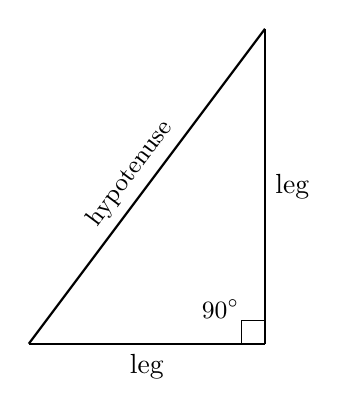
\begin{tikzpicture}
        \draw[thick] (0, 0) -- (3, 0) node[midway, below] {leg};
        \draw[thick] (3, 0) -- (3, 4) node[midway, right] {leg};
        \draw[thick] (3, 4) -- (0, 0) node[midway, sloped, above] {\small{hypotenuse}};
        \draw (2.7, 0) -- (2.7, 0.3) -- (3, 0.3);
        \node[above left] at (2.8, 0.2) {\small{$90^\circ$}};
    \end{tikzpicture}
\end{figure}

\section*{The Pythagorean Theorem}

The Pythagorean theorem states that in a right triangle, the square of the length of the hypotenuse is equal to the sum of the squares of the lengths of the other two sides.

The Pythagorean theorem can be written as: \boldmath$a^2 + b^2 = c^2$\unboldmath

where:
\begin{itemize}
    \item \( a \) and \( b \) are the lengths of the legs.
    \item \( c \) is the length of the hypotenuse.
\end{itemize}

If you draw squares on each of the three sides of the triangle, the sum of the areas of the two smaller rectangles equals the area of the square on the hypotenuse.

\begin{figure}[h!]
    \centering
    \begin{tikzpicture}
        \draw[thick] (0, 0) -- (3, 0) node[midway, below] {$a$};
        \draw[thick] (3, 0) -- (3, 4) node[midway, right] {$b$};
        \draw[thick] (3, 4) -- (0, 0) node[midway, left] {$c$} node[midway, sloped, below] {\tiny{hypotenuse}};
        \draw (2.7, 0) -- (2.7, 0.3) -- (3, 0.3);
        \node[above left] at (2.8, 0.2) {\tiny{$90^\circ$}};
        \draw[thick] (0, 0) -- (0,-3) -- (3,-3) -- (3, 0); \node at (1.5,-1.5) {$a^2$};
        \draw[thick] (3, 0) -- (7, 0) -- (7, 4) -- (3, 4); \node at (5, 2)     {$b^2$};
        \draw[thick] (0, 0) -- (-4,3) -- (-1,7) -- (3, 4); \node at (-0.5,3.5) {$c^2$};
    \end{tikzpicture}
    \\ \boldmath \Large{$a^2 + b^2 = c^2$} \unboldmath
\end{figure}

\newpage

\section*{Examples}

\subsection*{Example 1}

Given a right triangle with legs of lengths 3 and 4, find the length of the hypotenuse.

\textbf{Solution:}

Using the Pythagorean theorem:
\[
a^2 + b^2 = c^2
\]

Substitute \(a = 3\) and \(b = 4\):
\[
3^2 + 4^2 = c^2
\]

Calculate:
\[
9 + 16 = c^2
\]
\[
25 = c^2
\]
\[
c = \sqrt{25} = 5
\]

\textbf{Length of the hypotenuse:} 5

\subsection*{Example 2}

Given a right triangle with one leg of length 5 and a hypotenuse of length 13, find the length of the other leg.

\textbf{Solution:}

Using the Pythagorean theorem:
\[
a^2 + b^2 = c^2
\]

Substitute \(a = 5\) and \(c = 13\):
\[
5^2 + b^2 = 13^2
\]

Calculate:
\[
25 + b^2 = 169
\]
\[
b^2 = 169 - 25
\]
\[
b^2 = 144
\]
\[
b = \sqrt{144} = 12
\]

\textbf{Length of the other leg:} 12

\section*{Practice}

Solve the following problems using the Pythagorean theorem:

\subsection*{Problem 1}

A ladder is leaning against a wall. The bottom of the ladder is 6 feet away from the wall, and the ladder reaches a height of 8 feet on the wall. Find the length of the ladder.

\textbf{Solution:}

Using the Pythagorean theorem:
\[
a^2 + b^2 = c^2
\]

Substitute \(a = 6\) and \(b = 8\):
\[
6^2 + 8^2 = c^2
\]

Calculate:
\[
36 + 64 = c^2
\]
\[
100 = c^2
\]
\[
c = \sqrt{100}
\]
\[
c = 10
\]

\textbf{Length of the ladder:} 10 feet

\newpage

\subsection*{Problem 2}

A rectangular field has a width of 9 meters and a diagonal length of 15 meters. Find the length of the field.

\textbf{Solution:}

Using the Pythagorean theorem:
\[
a^2 + b^2 = c^2
\]

Substitute \(a = 9\) and \(c = 15\):
\[
9^2 + b^2 = 15^2
\]

Calculate:
\[
81 + b^2 = 225
\]
\[
b^2 = 225 - 81
\]
\[
b^2 = 144
\]
\[
b = \sqrt{144}
\]
\[
b = 12
\]

\textbf{Length of the field:} 12 meters

\end{document}
